% this file is called up by thesis.tex
% content in this file will be fed into the main document
\ifpdf
    \graphicspath{{4/figures/PNG/}{4/figures/PDF/}{4/figures/}}
\else
    \graphicspath{{4/figures/EPS/}{4/figures/}}
\fi

%: ----------------------- name of chapter  -------------------------
\chapter{Application of proposed method to object tracking on a mobile device} % top level followed by section, Recently

Recently, more and more powerful mobile devices become publicly available. Every next iteration increases the CPU speed and memory size. However, there is still a significant dearth of resources on the mobile devices as compared to the desktop machines, especially when it comes to the CPU power. Yet, many consumer-level devices start to include a graphical processing unit that is capable of rapidly performing parallel programming. In this section, we show how our learning method can be implemented on the mobile device for the challenging purpose of object tracking. The simplicity and speed of our method, combined with original simple features proposed in the section, allow us to develop a tracking algorithm that performs in near real time. This shows the feasibility of using out method for real-world applications in image processing.
\section{Resources available on the mobile device: iPhone 4S}
\subsection{Overview}
As our target mobile device, we have chosen the latest iteration of the popular iPhone brand: iPhone 4S. Our choice was partially guided by the fact that the device itself, and the means to program it were readily available and the programming lay well within our area of expertise. Much more important, however, was the possibility of harnessing the power of GPU, thereby increasing the speed of the parallel computations.
\begin{figure}[t]
		\centering
		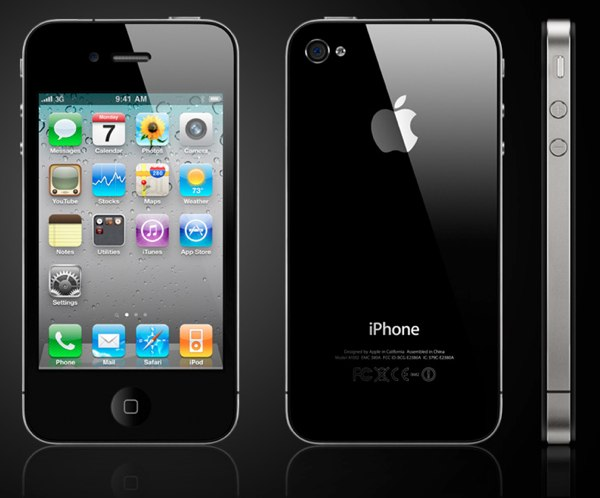
\includegraphics[width=0.7\textwidth]{iphone4s}
		\caption{iPhone 4S}
		\label{iph}
	\end{figure}
iPhone 4S is a touch-screen based smartphone released by Apple in the fall of 2011. It's design is similar to that of it's predecessor, iPhone 4 (see \figref{iph}). Its processing capabilities consist of the Apple A5 system-on-a-chip, that contains a dual-core ARM Cortex-A9 MPCore CPU, that includes NEON SIMD coprocessor for vector operations on the floating-point values, running at 1Ghz, image signal processing unit, performing such operations as face detection, white balance and image stabilization, and most importantly to us, an Imagination Technologies PowerVR SGX543 dual-core  graphics processing unit. Unfortunately,  the direct access to the ISP unit is limited to the system software, so it cannot be used or programmed to increase image processing speed, leaving us to rely on GPU only.

This phone demonstrates the increasing speed with which consumer-level mobile devices approach the capabilities of desktop computers. In fact, this a starling example of the Moore's law, since the processing capabilities of iPhone 4S are nearly double of its predecessor of only a year prior.

Latest versions of the iPhone system software (iOS 4 and 5) support the OpenGL 2.0 graphics library, which removes the fixed graphics pipeline, and introduces programmable vertex and fragment shaders, which allow not only a variety of imaging and video effects, but also to some extent general data processing in parallel. 

\section{General-purpose computing on graphics processing units}

General-purpose computing on graphics processing units (GPGPU) is the means of using a graphics processing unit (GPU), which typically handles computation only for computer graphics, to perform computation in applications traditionally handled by the central processing unit (CPU). 
 GPGPU requires a specific combination  between hardware components and software that allows the use of a traditional GPU to perform computing tasks that are extremely demanding in terms of processing power. Different GPU have different capabilities in that regard, with the GPUs for desktop video card allowing more flexibility and even the usage of a programming language developed specifically for GPGPU, while GPU on the mobile devices still offer only a limited programming capacity.  

General purpose computing on the GPU has greatly benefited from the new architectural approach GPU manufacturers have taken in their latest GPUs. In specific, these new GPU architectures come with a high grade of programmability, something not previously found in older generations of GPU architectures. Thanks to its broader range of programmability, the graphics processing unit has now been opened up to many kinds of applications and code.

Although GPGPU attempts were made in the past, they weren't very successful primarily because previous GPU architectures were very difficult to program for parallel processing. 

The effectiveness of the GPU usage largely depends on application. Tasks that are similar to graphics processing, that is, massively parallel, with low to none interdependency between the values being calculated. 
Usually, a certain amount of interaction between CPU and GPU is beneficial to the program's performance, however, one must always keep in mind that on most systems transfer of data between CPU and GPU memory is very slow, creating a programming bottleneck. 

As we have already established, GPUs are particularly well suited for parallel processing, a situation typically found in  image processing, generic patterns analysis, search for oilfields and natural resources, and analysis of financial risk calculation patterns. On the other hand, using GPUs for databases, data compression, recursive algorithms, and processes that require a high logical control of calculation is not ideal. A traditional CPU architecture would be far more efficient in this situation.

Unfortunately,  the low-power devices like iPhone do not benefit from the advantage of specially developed GPGPU languages, like CUDA or Cg. This means that we have to explore the programmable capabilities of the shaders in the graphics pipeline, while dealing with severe limitations described in detail below. 

\subsection{Open GL ES programmable graphic pipeline}
\begin{figure}[t]
		\centering
		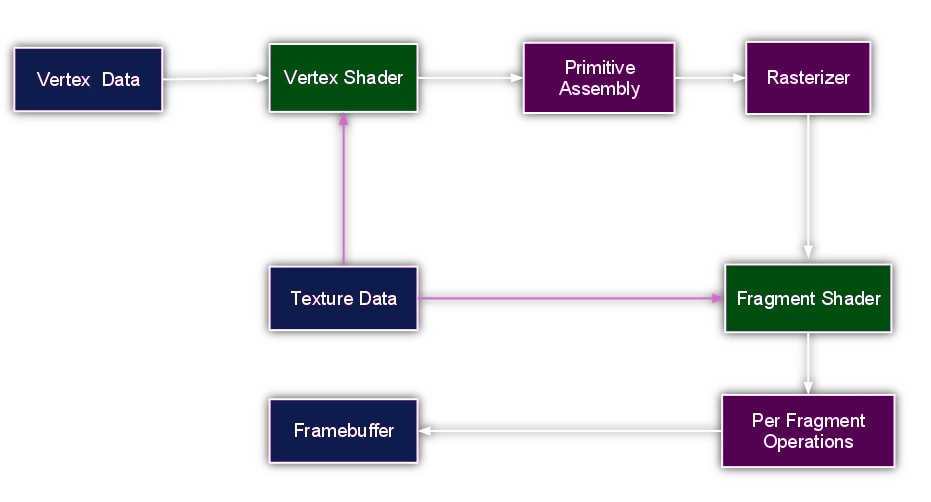
\includegraphics[width=0.7\textwidth]{glespipe}
		\caption{OpenGL ES programmable graphic pipeline (simplified)}
		\label{pipe}
	\end{figure}
OpenGL ES is a version of OpenGL graphics library for use on the mobile devices. Starting from OpenGL ES 2.0, it has received a complete overhaul, and for the first time has enabled usage of programmable graphics pipeline on the mobile devices.  While before, only some parameters of the graphic processing were available to change , OpenGL ES 2.0 added the ability of adding small programs called shaders (due to their original usage for achieving various shading effects), that are executed on GPU at key points during the graphic rendering process. The graphic processing pipeline is illustrated on \figref{pipe}

More specifically, ES 2.0 standard allow the usage of the so called vertex and fragment shaders. Vertex shaders are programs that are called once for each rendered vertex, and allow certain parameters to be interpolated between vertices on the same primitive. When applied for general calculations, they are generally used to set up environment for the fragment shader.

A fragment shader is called once per fragment, which usually corresponds to a single pixel on the screen or texture. Therefore, this is the shader where the majority of the parallel processing takes place. However, there are several limitations to the usage of the shader program, not the least of which being that a single shader can only produce a single 4-byte output  as of OpenGL ES 2.1. 

\begin{figure}[t]
		\centering
		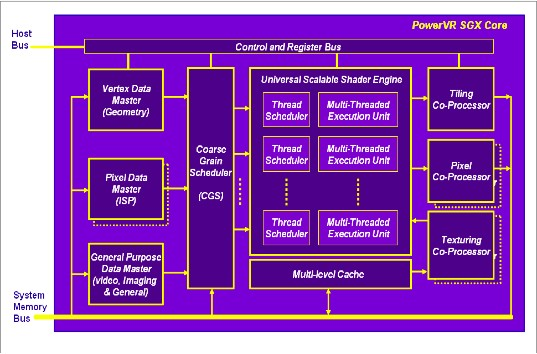
\includegraphics[width=0.7\textwidth]{GPUScheme}
		\caption{PowerVR SGX GPU architecture schematics}
		\label{gpu}
	\end{figure}
However, as can be seen from the illustration of the GPU architecture on \figref{gpu} , the advantage in using shaders lies in the fact that a large amount of them are executed at the same time, significantly reducing computational times for similar operations. 
\subsection{GPUImage programming library}
In our work, we use GPUImage programming library for iOS, written in Objective C. While in general, attaching and switching shaders is a relatively complex programming task due to an amount of auxiliary OpenGL code, the use of this library allows us to simplify and  streamline what would otherwise be nearly impossible to program by exposing a simple and user-friendly API. 

 The GPUImage framework is a BSD-licensed iOS library that lets you apply GPU-accelerated filters and other effects to images, live camera video, and movies. This library is available as an open source project on \href{https://github.com/BradLarson/GPUImage}{Github}, and allows us to express image processing tasks as a series of completely customizable filters that can be written using the OpenGL Shading Language. In our work, we develop several filters specific for our application, and also make use of several simple filters that are already available.

In particular, we make use of the following built-in filters: 
\begin{itemize}
 \item  GPUImageBlendFilter
 \item   GPUImageCropFilter
 \item GPUImageFastBlurFilter
 \item GPUImageRotationFilter
\end{itemize} 
Also, we make use of the video input exposed by the provided API. 

\subsection{Limitations}
\label{gpulim}
In this section, we outline several limitations of the OpenGL ES shader system,  as opposed to the GPGPU system available on desktop PC, and our adjustments to them.

\begin {itemize}
\item {\bf Lack of support for the floating point textures and limited precision}

The most important limitation is the fact that all highly parallel inputs and outputs in OpenGL ES are supposed to be textures, i.e. 2D arrays of data coded in, 4-byte vectors representing color. While desktop OpenGL allows the use of floating point textures, where the 4 bytes represent a single floating-point number of high precision or 2 of lower precision, OpenGL ES lack this feature, necessitating either recoding of incoming and outgoing data, which results in severe slowdowns rendering application useless, or working with low-precision data.

This precludes the GPU computation and usage of such tools as the integral image, which lead to the fact that such image features as Haar-like features and histogram-based features cannot be computed effectively. 
\item {\bf No support for preloaded render calls}

When it is necessary to perform a sequence of operations on the GPU, especially such series in which every consecutive step utilizes data output form the previous one, it would often be beneficial to store the sequence on the GPU before execution. In OpenGL ES, we, however, have to wait for each step to finish and inform CPU before starting the next one, significantly impacting performance. The only solution to this is to minimize the number of such operation series. 

\item {\bf No procedures available for linear (non-2D) arrays}

Once again, all operations on the mobile GPU are performed with textures serving as a data storage. In addition to the precision problems, there is little to no support for large one-dimensional arrays, necessitating packing such arrays into 2D form, thus adding unnecessary operations in the shader code. 

\item {\bf Opaque memory layout}

On the desktop, the layout of the memory available to each shader is well known, allowing to perform certain optimization techniques improving performance by efficient memory caching. In OpenGL ES, memory layout is more or less completely opaque. 

\item {\bf Insufficient tools for synchronization}

As was partially mentioned in the above point, possibly the only tool available for the synchronization between data operation in OpenGL ES is waiting for all GL render calls to complete. This decreases efficiency drastically. 

\item {\bf Relatively slow texture lookup}

 Looking up texel (texture element) values, especially when the coordinates are calculated in the fragment shader instead of being passed from vertex shader, is one of the most computationally expensive operations performed by GPU. Slow lookups limit the amount of pixel tests that can be performed while maintaining real-time processing speed.

\item {\bf Output constraints}

Output constraints. The outputs of each fragment (pixel) shader in the OpenGL ES programming framework have to fit into a single pixel of the output texture, i.e. 4 bytes of data in floating point format, which is reduced to four 8-bit integers. Furthermore, the precision of floating point operations and variations in the driver implementation does not allow access to individual bits of the output. 

\end{itemize}

\section{Modification of Pegasos algorithm for parallel processing}
\begin{figure}[t]
		\centering
		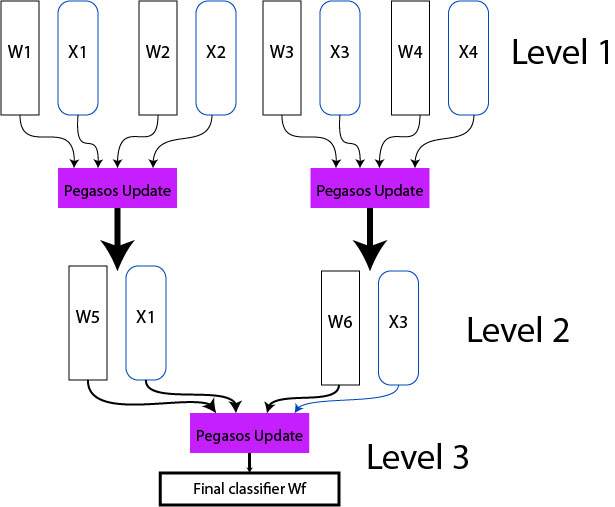
\includegraphics[width=0.7\textwidth]{pyrapega}
		\caption{Pyramidal Pegasos Algorithm}
		\label{pyra}
	\end{figure}
In this section we describe the modification to the Pegasos algorithm described in sec. \ref{pegaSec} for more efficient parallel processing, and compare it to the original.
\subsection{Modification description}
The original Pegasos algorithm was designed for sequential or batch-sequential updates, i.e. only allowing for a single or limited number of input samples $\vec{x},y$ per iteration. In the image processing task, however, we usually have the situation where a large number of input samples, possibly one for each pixel, is available at the same time when the frame is processed. One solution would be to just use all these inputs as a single batch, but that would decrease the efficiency of the algorithm.

Either way, for estimating the Pegasos update it is necessary to add the weighted value of misclassified sample together, which, while not a simple task for parallel processing, is relatively well developed (\cite{fung}). Therefore, based on the common algorithms for the parallel summations, we have developed a modification of the Pegasos algorithm which can be called Pyramidal Pegasos (\figref{pyra}). It uses the simple hierarchical scheme for summation, but in each step replaces summation with the following steps, assuming that each shader program has access to a sample vector and label pair $\vec{x}_i, y_i$, and a pair of weight vectors $\vec{w}_{i}$,$\vec{w}_{i+1}$ from the previous level(initialized at $\vec{0}$ on the first level):
\begin{enumerate}
\item Average the weight vectors $\vec{w}_o=\frac{1}{2}\left(\vec{w}_{i}+\vec{w}_{i+1}\right)$
\item Perform Pegasos update iteration (normal or weighted) on the vector $\vec{w}_o$ with $\vec{x}_i, y_i$
\item Output updated $\vec{w}_o$ to use in the next level 
\end{enumerate}
The result of the algorithm is a single vector of weights $\vec{w}$. It is easy enough to see that the amount of Pegasos updates performed is two times larger than in the case of sequential updates, but this expense is easily enough offset by the parallel processing gains. It is also possible to eliminate the first layer and distribute the data samples over layers , reducing the total number of updates to the number of input data samples.
\subsection{Evaluation}
In this section, we give a brief evaluation of the Pyramidal Pegasos modification, comparing its performance to the original Pegasos in order to determine whether we can use it in our application. For simplicity, we only evaluate the convergence on the linearly separable dataset. The results show that the convergence rate of this modifications is similar to the original algorithm. Unfortunately, the actual implementation of the algorithm on GPU with the use of OpenGL ES programming framework has shown us, that due to a large overhead associated with additional rendering calls for each pyramid level, the speed of the algorithm suffers in comparison to the CPU-only implementation. This drawback, however, is not present on the desktop GPU. Therefore , for the current version of our testing application, we have decided to use the standard sequential algorithm. However, we still consider this algorithm to be useful learning tool for the case of better optimized parallel implementation. 
\section{Simple local image features}

Due to the limitations of the OpenGL ES architecture and high computational cost, extraction of the global image features, even the simple features like Haar-like features (\cite{viola}) of local binary patterns(LBP) (\cite{LBP}) over large image region is unfeasible on the iPhone for any usable size of the region of interest, we had to develop our own set of features to estimate the feasibility of using our learning algorithm for image processing tasks.

The features that we use in our experiments a partially based on the same idea as Haar-like features and LBP, but extremely simplified to minimize the number of texture  fetches necessary. Essentially, where their features deal with image regions, ours mainly deal with singular pixels, possibly after passing the image through Gaussian filter for increased stability. We show, that even when using such features, our algorithm can provide a remarkable level of distinctiveness between image regions.

The feature vector for a single randomized feature is collected as follows:
\begin{enumerate}
\item For each feature, two random offsets $\vec{\Delta}_1$, $\vec{\Delta}_2$ are chosen
\item For each pixel with coordinate $\vec{p}$ in the ROI, luminance values of the pixels with coordinates $\vec{p}+\vec{\Delta}_1$ and $\vec{p}+\vec{\Delta}_2 $ are compared, and the result of comparison added as a feature
\item $r,g$, normalized color values for pixels at coordinates $\vec{p}$, $\vec{p}+\vec{\Delta}_1$ and $\vec{p}+\vec{\Delta}_2 $ are added to the feature vector.
\end{enumerate} 

As a result a single feature simply gives information of the color values of three pixels arranged in a certain configuration, and indicates whether one of the pixels in brighter than another, possibly indication an edge.

On its own, as single feature vector like that does not have much discriminative power, however, as we will show later, when several such features are combined using our proposed learning methods, they become capable of distinguishing a wide range of objects, although the performance is still inferior to the more robust global features. 
\section{Tracking}
In this work, we evaluate the applicability of the features described above combined with our learning method to image processing tasks. As an example task, inspired by \cite{OnlineBoost}, we have chosen simple object tracking. 

As shown in \cite{avidan}, object tracking on an image can be cast as a binary classification problem over a region of interest, separating an area containing object (usually a bounding box rectangle) from all other positions in the neighborhood. Some kind of movement model may be used to constrain the search area in order to reduce the amount of necessary computations. Also, since object changes from frame to frame, online adaptation can be used to update object model, as described in \cite{OnlineBoost}. Since our model is geared towards online learning, such updates are also possible, and their effect is investigated below.
\subsection{Training regime}
First, in order to separate object position from the surrounding background, an object model in the feature space have to be trained. Usually, this training is assumed to be done offline, after the original object position is . In our case, since we don't have a specific object, an area in the middle of the screen is trained as an object to be tracked. A ROI around the object position is selected, and a large amount of features are extracted and passed through a trainer with high learning rate set. Several pixels in the center of ROI are assumed to have label value of $1$, i.e. are assumed to be the true position of an object being trained, while all other pixels are assumed to have label value of $-1$. 

The large amount of negative samples compared to the positive ones creates an extremely imbalanced data set, which negatively affects the results of the learning algorithms based on gradient descent, like ours. In order to balance that, the positive samples are fed into algorithm multiple times. 

For this experimental application, we use a multiple feature modification of our algorithm described in section \ref{OurMethod}, with each new feature being randomly generated, as well as the removal of weak classifier due to the computational constraints of the mobile device.

\subsection{Position estimation}
After the initial model is trained, the application starts tracking the trained object, as well as continuously updating the model. In order to calculate the position of the object, we simply apply a threshold to the confidence function in the ROI, and calculate weighted average position on the remaining values. If all values are below threshold, the object is considered lost. This simple algorithm works reasonably well for many cases, although it has several drawbacks.
\section{Resulting Application layout}
\begin{figure}[t]
		\centering
		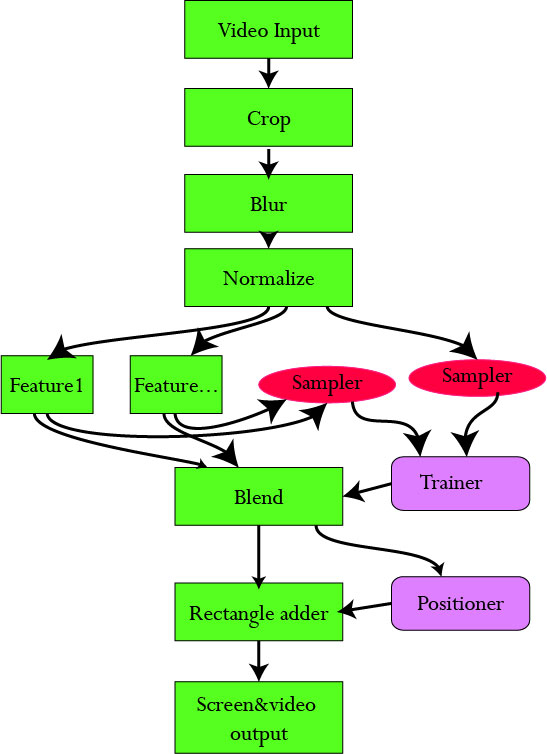
\includegraphics[width=0.9\textwidth]{tracking}
		\caption{Graphic filter layout used for tracking}
		\label{tracking}
	\end{figure}
The diagram on \figref{tracking} shows the resulting layout of the filters used by experimental application. The layers used are, in order
\begin{enumerate}
\item {\bf Input} An input texture uploaded from the iPhone video camera, at the resolution 640x480
\item {\bf Crop filter} Input image is cropped to an explained region of interest.
\item {\bf Blur filter} Cropped image is blurred by a low amount of Gaussian blur to increase stability.
\item {\bf Color normalization filter} The RGB values of each pixels are normalized to $rgl$, $l=\frac{R+G+B}{3}$, $r=\frac{R}{3*l+c}$, $g=\frac{G}{3*l+c}$, where $c$ is a small constant to prevent division by zero.
\item {\bf Feature sampler filter} A set of two filters sampling feature vectors from cropped image for the training of the current weak classifier. 
\item {\bf Weak classifier filters} A set of filters equal to the number of weak classifiers in the models that combine feature extraction and classifier evaluation.
\item {\bf Weak classifier extractors} A set of filters extracting calculated classifier values for training of the strong classifier.
\item {\bf A training block} Due to high accuracy demands exhibited by trainer, and GPU limitation, the actual trainings performed on CPU. With feature extraction and weak classifier estimation being performed in parallel, the computational demands of the algorithm itself are extremely low (more than 100K samples can be processed per second by our measurements). 
\item {\bf A multi-texture blending filter} Unlike other filter,this one has only a simple passthrough shader, instead achieving summation of the classifier outputs from the previous stage by  enabling built-in OpenGL blending and rendering all the input texture onto a single output. 
\item {\bf Position estimate block} This block uses output of the blend filter and calculates the position update of an object. Uses CPU. 
\item {\bf Rectangle filter} This filter simply add the rectangle on the estimated object position. 
\item {\bf Output} Output may be in form of the video file (movie encoder) or a screen output, or both. Since the CPU in this case is largely free of calculation, there is more than enough processing power for video compression. 
\end{enumerate}

\section{Results overview}
\begin{figure*}[t]
    \centering
\begin{subfigure}[b]{.45\linewidth}
       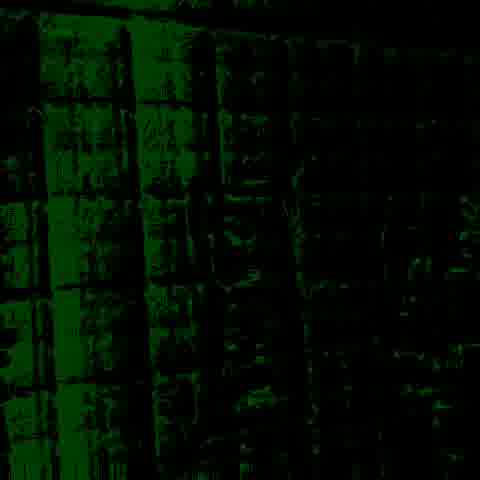
\includegraphics[width=0.9\linewidth]{conf1}
\label{startconf}
        \caption{Starting confidence map}
      \end{subfigure}%
\hspace{.01\linewidth}
\begin{subfigure}[b]{.45\linewidth}
	 
\includegraphics[width=0.9\linewidth]{conf2}
       \label{endconf}
      \caption{Converged confidence map}
  
	 \end{subfigure}%

 \begin{subfigure}[c]{.45\linewidth}
	   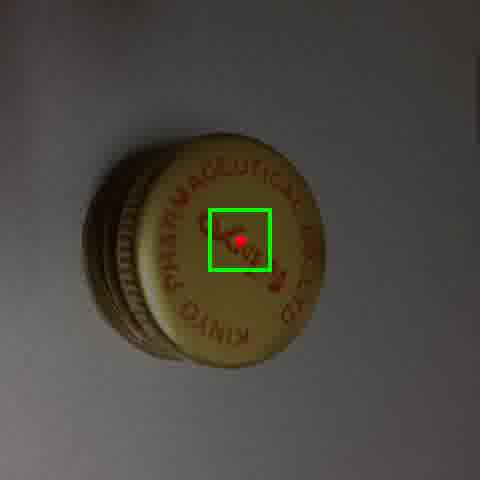
\includegraphics[width=0.9\linewidth]{track1}
           \label{tracking1}
           \caption{Tracking an object, starting position}
 \end{subfigure}%
\hspace{.01\linewidth}
\begin{subfigure}[c]{.45\linewidth}
    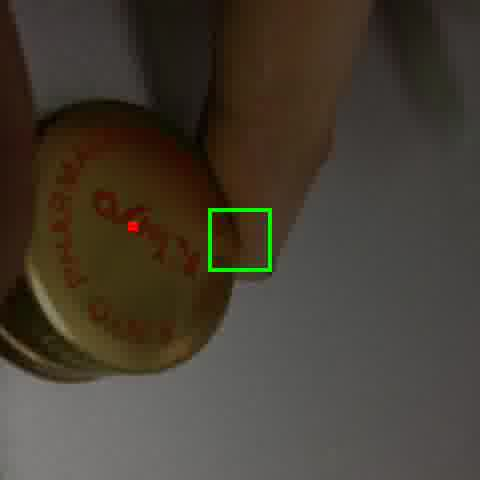
\includegraphics[width=0.9\linewidth]{track2}
    \label{tracking2} 
   \caption{Succesfully tracked an object}
\end{subfigure}%

\begin{subfigure}[c]{.45\linewidth}
	   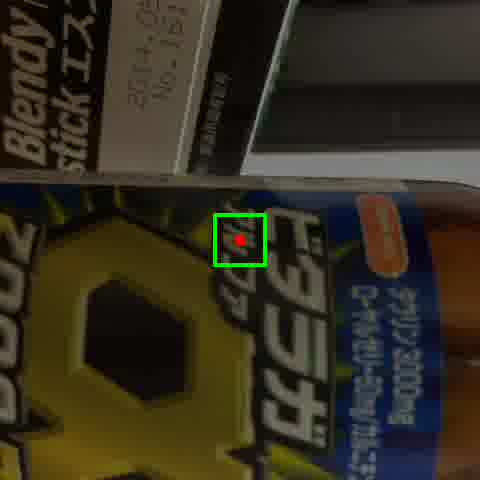
\includegraphics[width=0.9\linewidth]{tls1}
\label{lss1}
\caption{Tracking an ambiguous object}
\end{subfigure}%
\hspace{.01\linewidth}
\begin{subfigure}[c]{.45\linewidth}
	   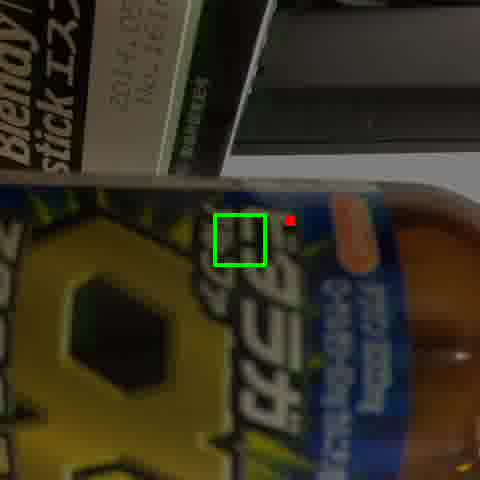
\includegraphics[width=0.9\linewidth]{tls2}
\label{lss2}
\caption{ Tracking lost}
\end{subfigure}%
    \caption{Some experimental results from tracking application}
    \label{trackim}
\end{figure*}
Some of the results of running sample application on the iPhone and attempting to define (segregate) and track various objects are illustrated on figure \figref{trackim}
The following conclusions can be drawn:
\begin{itemize}
\item The proposed features, while sufficient in many cases to separate object from the local background (Fig. \ref{trackim}\subref{endconf}, Fig. \ref{trackim}\subref{tracking2}), are not very robust due to the fact that they employ data from a low  number of pixels which may be noisy. They are also sensitive to scale and rotation. This sensitivity, combined with the fact that it is impossible to hold the phone absolutely steady while acquiring a target object, lead to the lower overall accuracy. 
\item Even with such limitations imposed by features and precision provided by GPU, the proposed learning algorithm can efficiently organize simple features to achieve object detection for the purposes of tracking, although the tracking is not very accurate (Fig. \ref{trackim}\subref{lss2}).  
\item The resulting algorithm is efficient enough to run in near real-time (12-17 fps) with the number of weak classifiers capped at 15.
\item However the simple position estimator suffers from the drawback of losing the tracked object when the movement exceeds its search area, while expanding search area leads to reduced efficiency of the classifier, since it has to offset the larger number of errors. 
\item The bottleneck of the algorithm appears to be a number of selectors, growing with the number of features. Repeated data transfers fro GPU to CPU memory, coupled with multiple rendering operations per selector reduce performance drastically. Removal of the need for them should nearly double the frame rate.
\item The learning algorithm is simple and efficient enough to be almost unnoticeable in terms of computational and memory requirements when compared to feature extraction and especially selectors.
\item The usage of online adaptive algorithms for tracking can actually decrease the tracker's quality, a fact mentioned in \cite{grabner2008} due to an effect called drifting, where a classifier essentially retrains itself to accept other objects by accumulating errors. Due to high adaptability of our algorithm on limited number of weak classifiers, and high sensitivity of the features used, this effect is quite prominent unless care is taken to avoid it. 
\end{itemize}

To conclude, while the proposed experimental application clearly shows the merit of our learning method as applied to the image processing tasks like object recognition and tracking due to its simplicity and efficiency, the application itself is of limited practical value due to several unresolved problems in implementation. As such, it can be considered a proof-of-concept application rather than a final product. 



\section{Extending classification method to work with different features}
It can be noted that our proposed simple features bear certain resemblance to Ferns features proposed in (\cite{Ferns1}, \cite{Ferns2}), though our features incorporate color information and only a single binary check. In this section we show how this similarity allows us to enhance and widen the application of existing classification method by applying the boosting paradigm to it.
 We then demonstrate the implementation of modified algorithm on the mobile device.
\subsection{Introduction of Ferns}
\label{Intro}
Introduced by  Ozuysal et. al, Ferns use non-hierarchical structures consisting of a small number of random binary tests to estimate probability of an image patch belonging in a certain class.
Since the recovery of a full joint distribution of a large number of features (typically about 400) is not feasible, they propose separating a set of features of a large size N into M subsets of size $S=N/M$, choosing M in such a way that joint posterior distribution over S features can be recovered. Each subset is then assumed to be independent from all other subsets, which allows them to combine posterior probabilities by using naive Bayesian approach: 
\begin{equation}
\label{naive}
P(f_1,f_2,...,f_N|C=c_i)=\prod_{k=1}^{M}P(F_k|C=c_i)
\end{equation}
where $P(f_1,f_2,...,f_N|C=c_i)$ is conditional probability over features $f_i$ and $P(F_k|C=c_i)$ are probabilities of ferns $F_k$ estimated from training values. Since ferns employ binary features, values of ferns are encoded as an integer in binary representation, $F_m=\sum_{i=0}^{S-1}2^i f_{m*S+i}$. Each fern can then take values from 0 to $K=2^S-1$ The end result is semi-naive Bayesian approach, which models some but not all dependencies between features. 
The training phase of Ferns estimates the class conditional probabilities for each Fern $F_m$ and each class $c_i$(represented by a set of affine transformations of the image patch around corresponding keypoint). For estimation of probabilities, \cite{Ferns1} used uniform Dirichlet prior, resulting in a formula 
\begin{equation}
\label{approxD}
\hat{P}(F_m=k|C=c_i)=\frac{N_{k,c_i}+1}{N_{c_i}+K+1}
\end{equation}, where $N_{k,c_i}$ is the number of test samples in class $c_i$ for which $F_m=k$, and $N_{c_i}$ is the total number of members of that class in the training set. This prevents zero-valued probability estimates.
During classification, the binary features are extracted for each keypoint on the input image $\vec{I}$, and each keypoint is classified according to maximum likelihood or discarded if the maximum likelihood is too low: 
\begin{equation}
\label{estim}
\hat{c}_i=\argmax_{c_i}{P(f_1,f_2,...,f_N|C=c_i)}
\end{equation}
Since a large number of affine transformations of an image patch are used for probability estimation, the resulting distribution is independent of pose and lightning conditions, allowing a simple and efficient classification at run-time.
This algorithm has been successfully adapted to mobile tracking problem in \cite{Mobi}, however, it has been noted that its accuracy is degrading rapidly as the number of features decreases.

\subsection{Algorithm description}
\label{malg}
In this section, we derive our modification for a simple case of binary classification. The modified algorithm can then be used for such tasks as pose-independent texture recognition (further explored in section \ref{implementation}) or background extraction.
In our algorithm, we also use subsets of binary features for estimating joint conditional probabilities. The estimation process is in general similar to the one described in section \ref{Intro}, though it can be adapted depending on the applications. Some examples of the adaptation are described in section \ref{implementation}.  The main difference lies in combination of the estimated joint probabilities. While Ferns use a sum of log-likelihoods
\begin{equation}
\label{logsum}
log(P(f_1,f_2,...,f_N|C=c_i))=\sum_{k=1}^{M}log(P(F_k|C=c_i))
\end{equation}
we explore the possibility of weighting the likelihoods. Specifically, the formula for final likelihood for class $I$ is as follows:\begin{equation}
\label{norsum}
L(f_1,...,f_N,c_i)=\sum_{k=1}^{M}w_k l(F_k,c_i)
\end{equation}
where $L(f_1,...,f_N,c_i)$ is estimated likelihood and $l(F_k,c_i)$ can be one of the three functions: 

Function 1. The joint probabilities themselves:$l(F_k,c_i)=P(F_k|C=c_i)$ ,

Function 2. The logarithms of joint probabilities: $l(F_k,c_i)=log(P(F_k|C=c_i))$,

Function 3. The binary-thresholded probabilities, 1 for the class with maximum joint probability over selected features, and -1 for all others: $l(F_k,c_i)= \left\{ \begin{array}{rl}
1 &\mbox{ if } c_i=\argmax_{c_i}{P(F_k,c_i)} \\
-1 &\mbox{ otherwise}
\end{array} \right.$


All three functions have their own advantages and disadvantages. Using Function $2$ results in the model closest to naive Bayesian, with the weights more or less than one roughly representing positive and negative values of Spearman’s rank correlation between a given fern and all others for a certain class. The training, however, has a slightly larger performance cost, which has to be taken into account if the likelihoods are updated during classification. Use of Function $1$ has the least calculation cost, but has little theoretical basis.   Use of Function $3$ is ess performance-intensive option that sacrifices additional information present in Functions $1$ and $2$, but can provide memory savings up to a factor of 8. Our experiments in \ref{exp1} show that in case the training is done offline, Functions $1$ or $3$ in general provide better accuracy over Function $2$, with no additional cost at the classification stage. 
If we consider Function $3$ for the binary case, we can see that it reduces original problem to a set of semi-independent binary classifiers, which have to be linearly combined into a stronger (also binary) classifier. This is a classical definition of the binary boosting problem. We then use the online support vector machine training methods described in detail in chapters \ref{Chap2} and  \ref{OurMethod}. In particular, for this problem we use NORMA (\cite{Norma}) over Pegasos (\cite{Pegasos}) method to further simplify implementation, with the input vectors consisting of $\vec{x_i}=(l(F_1,c_i),l(F_2,c_i),...,l(F_S,c_i))$, with different values of $l(F_k,c_i)$ as defined for Functions $1$, $2$ and $3$, correspondingly. 

\subsubsection{Adding color information}
The original Fern formulation in \cite{Ferns1}, as well as many algorithms for keypoint and texture recognition, operates on the greyscale images, completely ignoring color information provided by most image sensors of mobile phones these days. This is less important for the keypoint classification, since most of the keypoints are by default located in the region of varying intensity, near the edges or corners. If we consider texture or object recognition problem, color becomes much more important, since the texture to be recognized may contain large uniform areas, and only differ in color from the background.  As a solution, we propose slight modification to the Fern binary checks. Instead of simply comparing intensities of two pixel with random offsets, each check is represented by the following formula:
\begin{equation}
\label{funct}
f_i=I(r(\vec{I}(\vec{x}+\Delta \vec{x}_0))\pm r(\vec{I}(\vec{x}+\Delta \vec{x}_1))>0)
\end{equation}
where $\vec{I}(\vec{x}+\Delta \vec{x}_0)$ and $\vec{I}(\vec{x}+\Delta \vec{x}_1)$ are 3-component color vectors for the feature offsets $\Delta \vec{x}_0$ and $\Delta \vec{x}_1$, correspondingly, $r(\vec{c})=(\vec{z},\vec{c})$, $\vec{z}={z_i}$, $i=1..3$ is a vector with randomly selected coefficients, and $I(cond)$ is indicator function. Depending on the sign in the equation \ref{funct}, it can have what we call symmetrical (for +) and antisymmetrical (for -) forms. In order to preserve validity of the features, coefficients $f$ for symmetrical features are selected so that $\sum_{i=1}^{3} {z_i}=0$. Several training experiments indicate that during training, Ferns containing mainly symmetrical or antisymmetrical features have larger resulting absolute values of SVM coefficients depending on whether the training area is flat or contains obvious intensity changes, correspondingly. This shows that the best ferns for a given pattern or keypoint can be selected by discarding ferns (and corresponding features) with the lowest $w_k$ and adding newly selected random features.

Training, then, can proceed in two ways. 1. The separate training. SVM weights are calculated after the joint probabilities have been estimated for all poses and texture positions. The advantages of this method include increased accuracy due to more precise probability estimates. The disadvantages are that either the features have to be extracted two times or the input vectors have to be saved, requiring higher memory consumption. 2. Interleaved training consists of adding each feature vector to both histogram for probability estimation and then SVM, according to eq. \ref{NORMAUpdate}. This allows processing all input data in a single pass, and depending on implementation may allow for online adjustments, allowing model to change depending on the detected pattern. 


\subsubsection{Multiple classes}
\label{multiclass}
While the focus of our work is on binary classification, most problems in image processing are not confined to only two classes. The keypoint recognition problem, for instance, can easily have several hundred detected keypoints, resulting in a large amount of classes. 
From eq. \ref{NORMAUpdate} it can be seen, that in linear case, NORMA training weights are altered in a way that changes value of the testing function in the direction of correct classification. This change only happens if the training vector is misclassified or lies within margin. Based on this, the update step for multiple classes can be formulated in a way that, in case of misclassification, estimated likelihood is reduced for the wrong class while it is increased for the correct class. The example of update step is then:
\begin{equation}
\begin{array}{l}
\hat{c}_k=\argmax_{c_t}{ (\vec{w}_{i},\vec{l}_{c_t})}\\
\hat{c}_s=\argmax_{c_t\ne\hat{c}_k}{ (\vec{w}_{i},\vec{l}_{c_t})}\\
\alpha_i=\left\{ \begin{array}{rl}
0 &  c_k=c_i \mbox{ \&\& } (\vec{w}_{i},\vec{l}_{\hat{c}_k})-(\vec{w}_{i},\vec{l}_{\hat{c}_s})>1 \\
1 & \mbox{otherwise}
\end{array} \right.\\
\vec{w}_{i+1}=(1-\eta_i \lambda )\vec{w}_i +\alpha_i \eta_i (\vec{l}_{c_i}-\rho \vec{l}_{c_k}) \\
\end{array}
\label{multic}
\end{equation}
where $\rho$ is an additional parameter regulating ratio between the gradients for the correct and the incorrect classifications. 
\subsection{Offline experiments}
\label{exp1}
In our experiments, we mainly concentrate on the task of binary texture recognition that we use for further implementation on the mobile device.
For that, we select an image with a known textured area and train original Ferns as well as SVM-boosted Ferns by creating histograms of probability distributions for texture and background classes. This includes affine transformations of patches taken from both areas to make resulting marginal distribution pose-independent. We evaluate the accuracy by classifying several test images, for which the ground truth values were given by hand, and evaluating the ratio of misclassified pixels to the total number of pixels.


\begin{figure*}[t]
    \centering

\begin{tabular}{l| c| c| c }
{\raisebox{0.75in}{Image set 1}} &
{
	 \begin{subfigure}[b]{.25\linewidth}

	   
\includegraphics[height=1in]{images/tb2.jpg}

\caption{}	 
\label{s1}
 \end{subfigure}}
&
{
	 \begin{subfigure}[b]{.25\linewidth}
	   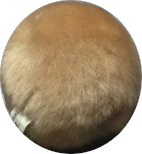
\includegraphics[height=1in]{images/t2.jpg}

\caption{}
\label{s2}
	 \end{subfigure}}&
{
  \begin{subfigure}[b]{.25\linewidth}
	   
\includegraphics[height=1in]{images/test1.jpg}

\caption{}
\label{s3}
	 \end{subfigure}}
\\[0.3in]

{\raisebox{0.75in}{Image set 2}}
&
{
 	 \begin{subfigure}[b]{.25\linewidth}
	   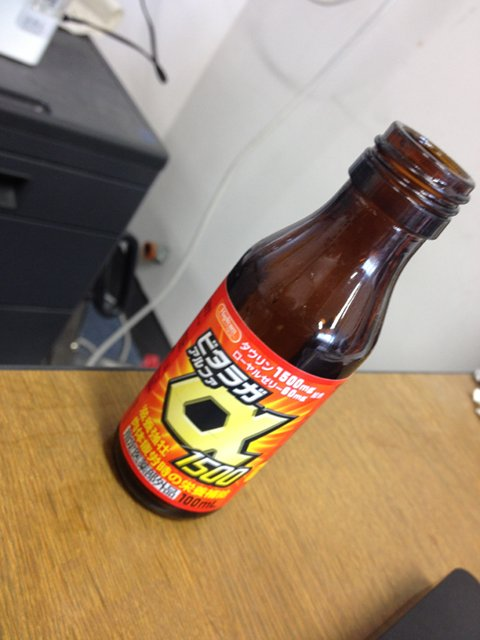
\includegraphics[height=1.5in]{images/train1.jpg}

\caption{}
\label{s4}
		 \end{subfigure} }
&{
\begin{subfigure}[b]{.25\linewidth}
	   
\includegraphics[height=1.5in]{images/ttext1.png}

\caption{}
\label{s5}
	 	 \end{subfigure}}
&{
\begin{subfigure}[b]{.25\linewidth}
	   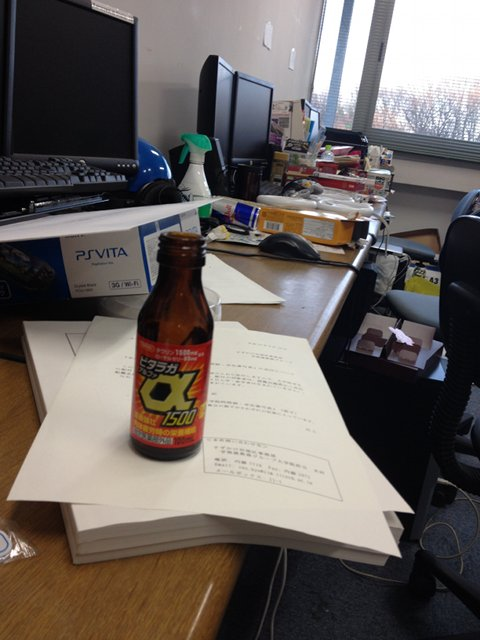
\includegraphics[height=1.5in]{images/test2.jpg}

\caption{}
\label{s6}
	  \end{subfigure}}

\end{tabular}
    \caption{Examples of training images and clipped textures. \protect\subref{s1} , \protect\subref{s4} Images used for training. \protect \subref{s2}, \protect \subref{s5}  Texture area extracted for training \protect \subref{s3}, \protect \subref{s6} Examples of the images used for evaluation.  
}
    \label{Samples1}
\end{figure*}
\begin{table}

\begin{tabular}{|c||c|c|c||c|c|c|}

                                                                            \hline
  {}  &  \multicolumn{3}{|c||}{Image set 1}  &\multicolumn{3}{|c|}{Image set 2}    \\\hline
    {}  & {\parbox[c][2.5em]{0.13\linewidth}{\centering\begin{spacing}{0.7} 6 bits, \linebreak 30 Ferns\end{spacing}}} & {\parbox[c][2em]{0.13\linewidth}{\centering\begin{spacing}{0.7} 8 bits, \linebreak 30 Ferns\end{spacing}}}& {\parbox[c][2em]{0.13\linewidth}{\centering\begin{spacing}{0.7} 8 bits, \linebreak 50 Ferns \end{spacing}}} &{\parbox[c][2em]{0.13\linewidth}{\centering\begin{spacing}{0.7} 6 bits, \linebreak 30 Ferns\end{spacing}}}  &{\parbox[c][2em]{0.13\linewidth}{\centering\begin{spacing}{0.7} 8 bits, \linebreak30 Ferns\end{spacing}}}&{\parbox[c][2em]{0.13\linewidth}{\centering\begin{spacing}{0.7} 8 bits,  \linebreak50 Ferns\end{spacing}}} \\\hline

 {log}  & {0.76} & {0.78}& {0.80} &{0.58}  &{0.57}&{0.58} \\\hline
 {prob}  & {0.51} & {0.52}& {0.61} &{0.5}  &{0.5}&{0.51} \\\hline
 {bin}  & {0.62} & {0.69}& {0.73} &{0.61}  &{0.61}&{0.63} \\\hline

  {wlog}  & {0.83} & {0.84}& {0.88} &{0.78}  &{0.81}&{0.90} \\\hline
 {wprob}  & {0.81} & {0.81}& {0.82} &{0.9}  &{0.9}&{0.92} \\\hline
 {wbin}  & {0.93} & {0.92}& {0.92} &{0.88}  &{0.89}&{0.92} \\\hline


{iwlog}  & {0.77} & {0.77}& {0.80} &{0.70}  &{0.75}&{0.80} \\\hline
 {iwprob}  & {0.60} & {0.63}& {0.75} &{0.81}  &{0.82}&{0.85} \\\hline
 {iwbin}  & {0.65} & {0.71}& {0.80} &{0.81}  &{0.83}&{0.85} \\\hline

\end{tabular}

\caption{Average ratio of successfully recognized pixels to the total number of pixels in the test images. Sample test images for the image sets 1 and 2 are presented on \ref{s3} and \ref{s6}, respectively.}
\label{tbl1}
\end{table}

We perform tests of different methods on the two sets of images, 3 480x640 RGB images each, with 1 image used for training and two images with differing texture poses used for testing (examples given in Figure \ref{Samples1}), comparing accuracy of original Ferns and SVM-boosted ferns for 3 values of $l(F_k,c_i)$, for both interleaved and separate training methods. The results of completed training are presented in table \ref{tbl1}. In the table $log$, $prob$ and $bin$ standing for likelihood functions $1$, $2$ and $3$, respectively, applied to original Ferns (no weighting), $wlog$, etc. refer to weighted Ferns using separate training, and $iwlog$, etc. to weighted Ferns using interleaved training.  It can be seen that all methods that use training provide increased accuracy over the original Ferns method, especially when the Ferns bit size and total amount of features are decreased. For particularly low values of fern size (below 6 bit), the binary method starts to outperform other methods of likelihood estimation. In the limit case, the method essentially becomes our original method for SVM boosting. This is useful for applications where the amount of storage is limited, since it allows storing each feature in single bits rather than floating point values. It should be noted that this increase of accuracy comes without any increase of computational cost during classification stage, since the likelihoods can be premultiplied by SVM coefficients in case of offline training, and multiplications replace logarithm calculation in case the online updates are used. 
To estimate the performance and accuracy of multiclass method, we perform the same tests as in the original Ferns article \cite{Ferns1}. The results are shown in Figure \ref{multires}. Our experiments have shown that while our algorithm outperforms the original on shorter Ferns and lower number of classes, benefits decrease as the amount of classes and available Ferns increases, indicating that for applications with larger available resources and stricter requirements to training times the original method could be preferable.

\begin{figure}[ht]
    \centering

	\begin{subfigure}[b]{.45\linewidth}
	   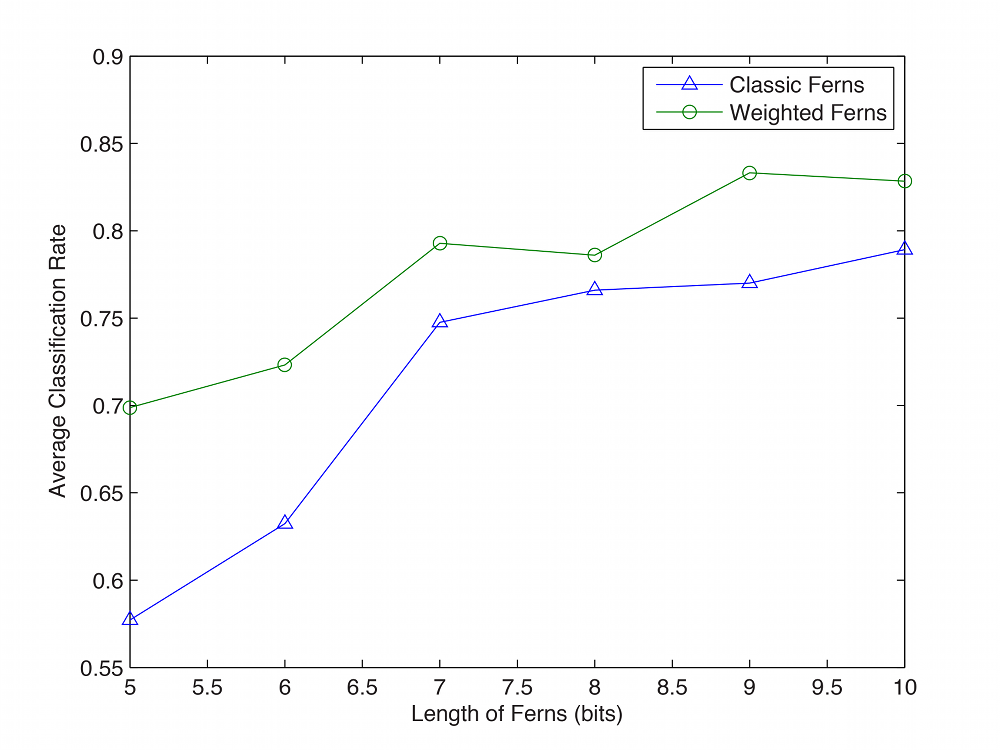
\includegraphics[height=2in]{images/fernlen.png}
\label{lenferns}
\caption{}
	 \end{subfigure}
	\begin{subfigure}[b]{.45\linewidth}
	   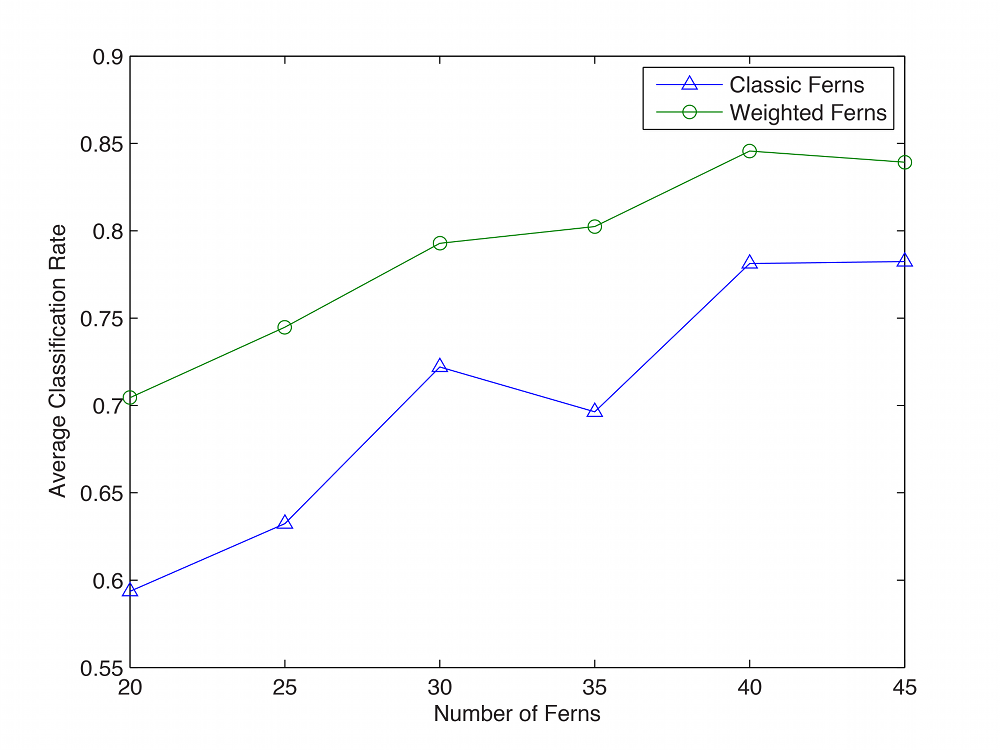
\includegraphics[height=2in]{images/fernnum.png}
\label{numferns}
\caption{}
\end{subfigure}
  \caption{Results of testing multiclass approach described in section \ref{multiclass} with 50 classes.  Ratio of correctly classified image patches to a total number of patches (accuracy ratio). \protect \subref{lenferns}  Dependence of accuracy ratio on a bit length of each Fern (25 Ferns total).  \protect\subref{numferns} Dependence of accuracy ratio on a total number of Ferns (8 bits per Fern).  }
\label{multires}
\end{figure}

\subsection{Mobile device implementation}
\label{implementation}
\begin{figure}[ht]

    \centering

	\begin{subfigure}[b]{.37\linewidth}
	   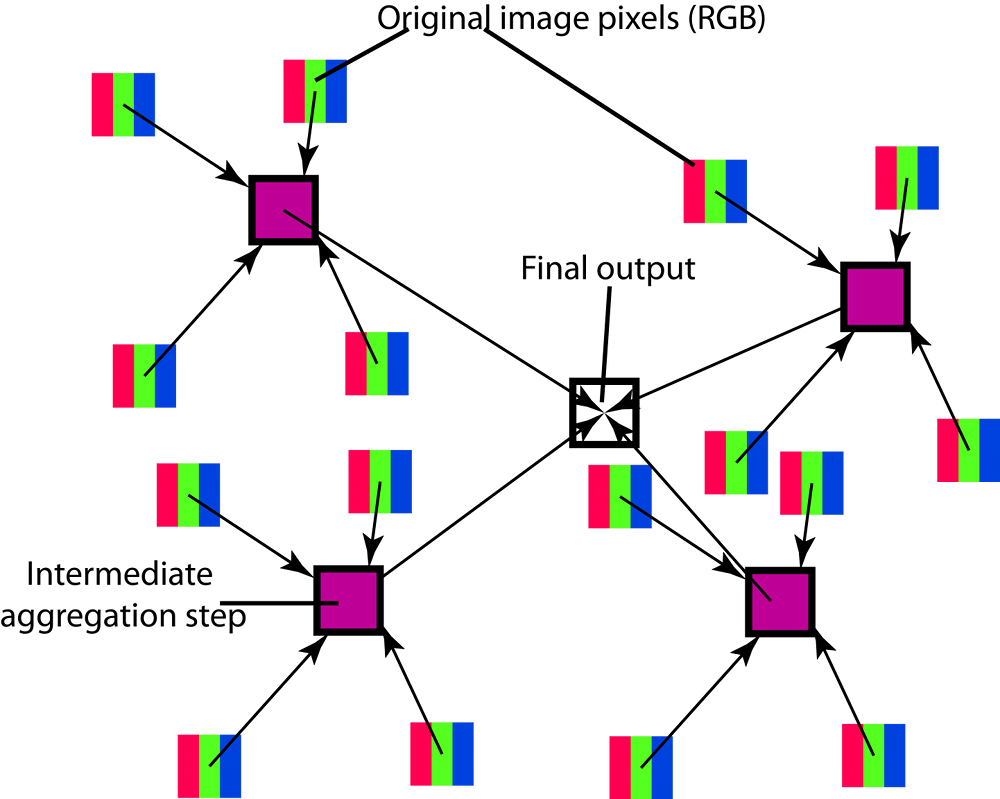
\includegraphics[height=1.7in]{images/Shader1c.png}
\caption{Illustration of multilevel data aggregation. Four RGB pixels are processed by first layer, resulting in the intermediate value (purple). The next shader in chain then processes four intermediate values, aggregating data from a total of 16 pixels, and gets the result of the second level(shown as a white square).}
\label{eps1}
\end{subfigure} 
	\begin{subfigure}[b]{.37\linewidth}
	   
\includegraphics[height=1.7in]{images/Shader2c.png}
\caption{Illustration of complete shader chain for likelihood estimation. Shader 1 calculates Ferns and looks up premultiplied binary values in an auxiliary lookup texture. Shader 2 aggregates outputs of Shader 1 into a single likelihood.}
\label{eps2}
\end{subfigure}

    \caption{ Illustration of shader layout for improved Ferns classification}
\label{shaders}
\end{figure}

Next, we show how to implement the texture recognition algorithm outlined in section \ref{malg}, based on two-class SVM-boosted Ferns. Its computation is performed mostly by GPU, with very little CPU participation. Since it allows estimating likelihood of a given pixel being part of texture are for every pixel of an image, the keypoint / region of interest detection step can be avoided.
At its core, the implemented algorithm is simple. Once the offline training is done, we have a set of probability distributions $\hat{P}(F_m=k|C=c_i)$ and corresponding weights $w_m$ for all Ferns, which can then be arranged into lookup tables and saved as reference textures in the video memory. To simplify uploading process, tables can be arranged and saved as PNG images beforehand (examples in Figure \ref{TSamples1}), or saved, for smaller number of Ferns, saved as text file. Then, for classification, the fragment shader has to perform necessary binary tests to create Ferns for each pixel (using eq.  \ref{funct}), form lookup indices and calculate the resulting likelihoods by summing over values fetched from lookup texture. Here, however, we run into several limitations of the OpenGL ES shader programming, as outlined in section \ref{gpulim}.

\subsection{Resulting algorithm}
\label{ra}
Our resulting algorithm uses chain of 2 shaders to transform original image into either likelihood estimation of each pixel belonging to an input texture or the thresholded value thereof.  The complete chain is illustrated in Figure \ref{eps2}. The chain uses two shaders. The first one calculates Fern values given pixel offsets used during training, and then recovers intermediate likelihood values from a lookup texture. In our case, each texel contains four values in four color channels available (RGBA), each value being either 0 (in case a Fern indicates background with greater likelihood) or 8-bit SVM coefficient for a corresponding Fern. The second shader sums outputs of the first one over the second set of predefined offsets, and outputs final likelihood of a given pixel belonging to a texture. An additional shader is then used to blend the likelihoods with original image for visualization. As can be seen, all of the image processing is completely performed on the GPU, freeing up CPU for additional tasks, such as possible online model training.

\begin{figure}[ht]
    \centering
\begin{minipage}[b]{.3\textwidth}
	 \begin{subfigure}[b]{.4\linewidth}
	   
\includegraphics[height=1.8in]{images/fernUnpacked1.png}
\caption{}
\label{ts:scr1}
	  \end{subfigure}
	
	 \end{minipage}
	 \begin{minipage}[b]{.3\textwidth}
 \begin{subfigure}[b]{.4\linewidth}
	   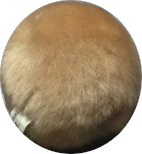
\includegraphics[height=0.9in]{images/t2.jpg}
\caption{}
\label{ts:scr3}
	 \end{subfigure}\\
\begin{subfigure}[b]{.4\linewidth}
	   
\includegraphics[height=0.9in]{images/backgrounds.jpg}
\caption{}
\label{ts:scr4}
	\end{subfigure}
	 \end{minipage}

    \caption{Weights and thresholded probabilities for 16 Ferns encoded  in a PNG image  (\protect \subref{ts:scr1}  for loading in mobile device. Each 16x32 rectangular region encodes a single 9-bit Fern (512 possible values).  \protect \subref{ts:scr3} Texture used for training \protect \subref{ts:scr1}. \protect \subref{ts:scr4} Sample of background used for training \protect \subref{ts:scr1}}
    \label{TSamples1}
\end{figure}

\subsection{Implementation results}
\label{iresults}

\begin{figure}[ht]
    \centering

\begin{subfigure}[b]{.3\linewidth}
	   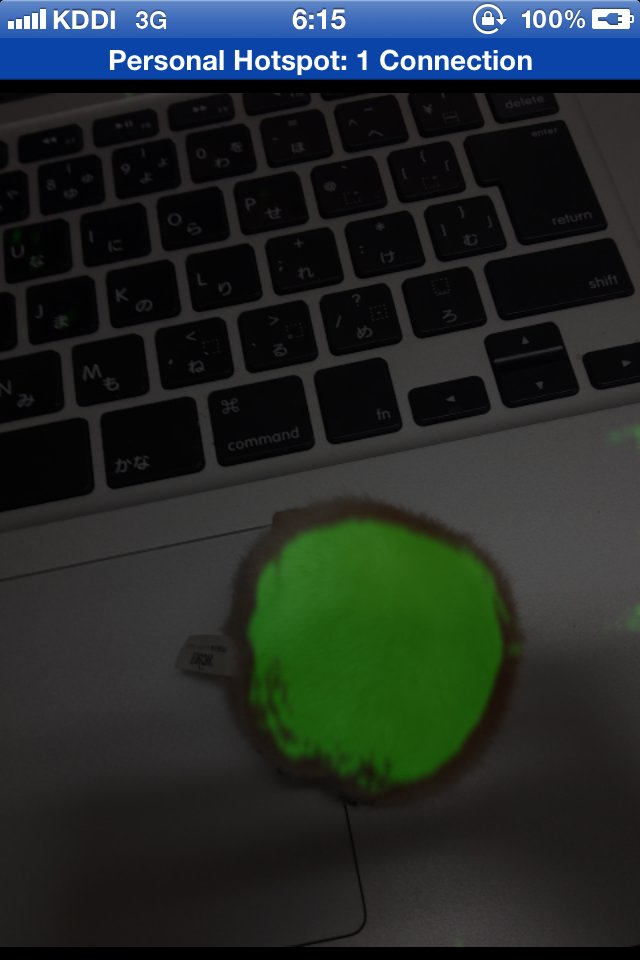
\includegraphics[width=0.9\textwidth]{images/IMG_1807.jpg}
\caption{}
\label{scre1}
	 \end{subfigure}
	\begin{subfigure}[b]{.3\linewidth}
	   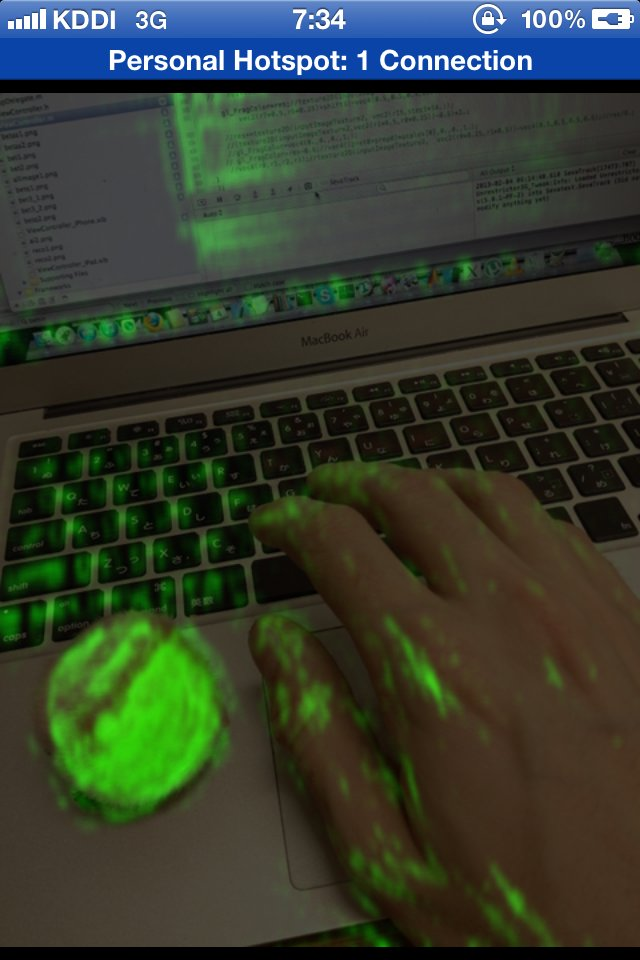
\includegraphics[width=0.9\textwidth]{images/IMG_1809.jpg}
\caption{}
\label{scre2}
	 \end{subfigure}
\begin{subfigure}[b]{.3\linewidth}
	   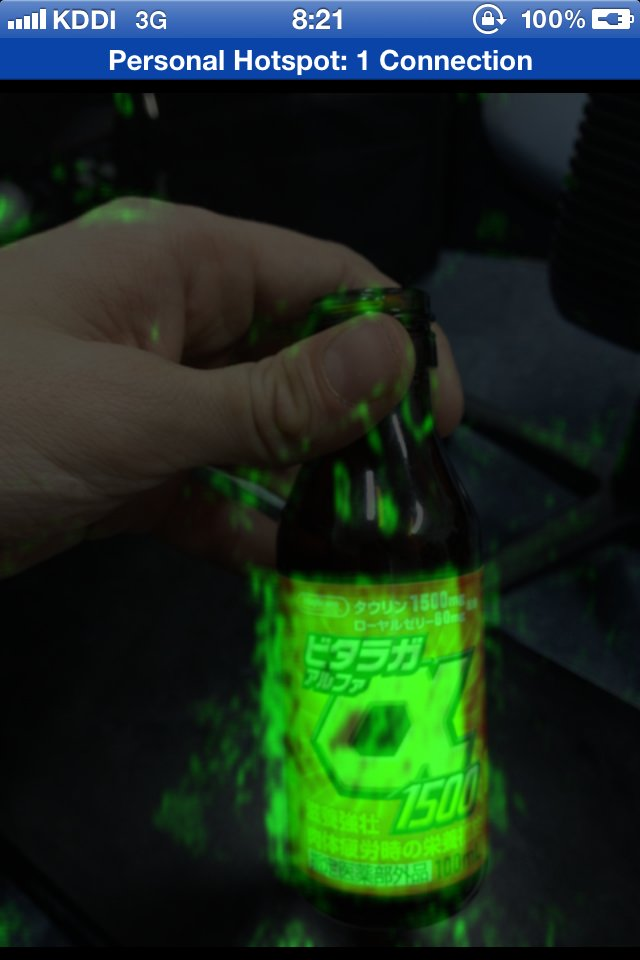
\includegraphics[width=0.9\textwidth]{images/IMG_1812.jpg}
\caption{}
\label{scre3}
	 \end{subfigure}
 

    \caption{Screenshots of texture recognition algorithm in operation. \protect \subref{scre1} , \protect\subref{scre2} are results of using weighted Ferns trained on texture from Figure \protect \ref{s2}, \protect \subref{scre3} uses method trained on  Figure \protect \ref{s5}. }
    \label{screenshots}
\end{figure}
Our algorithm with the above modifications was implemented on the iPhone4S. A built-in video camera, running at 30 fps with the resolution of 640x480, was used as source of input images. The two sets of images shown in Figure \ref{Samples1} were used separately  for training and recognition of the texture contained in each of them. The probability data from training was encoded in a set of PNG images each (example of an encoding image for 9-bit Ferns is presented in Figure \ref{TSamples1}, higher Fern length being used for improved clarity). For training, 64 9-bit ferns were used, and the joint distributions were then thresholded according to description in Section \ref{malg}. Since no ground truth values were available, the video was evaluated visually, and the speed of the algorithm was measured by averaging the time passing between frames. Several screenshots captured during the operation are displayed in Figure \ref {screenshots}. The average speed does not change with recognized texture, remaining stable at about 0.04 seconds per frame, that is, algorithm allows us to achieve 25fps for a relatively high-resolution video.  As can be seen, our algorithm achieves high recognition accuracy for the trained texture despite change of pose, and achieves real-time speeds while processing all of the image pixels. 


%: ----------------------- paths to graphics ------------------------

% change according to folder and file names


%: ----------------------- contents from here ------------------------







% ---------------------------------------------------------------------------
%: ----------------------- end of thesis sub-document ------------------------
% ---------------------------------------------------------------------------

